\documentclass[a4paper,10pt,conference]{ieeeconf}

\IEEEoverridecommandlockouts
\overrideIEEEmargins
\usepackage{graphics} % for pdf, bitmapped graphics files
\usepackage{epsfig} % for postscript graphics files
\usepackage{mathptmx} % assumes new font selection scheme installed
\usepackage{times} % assumes new font selection scheme installed
\usepackage{amsmath} % assumes amsmath package installed
\usepackage{amssymb}  % assumes amsmath package installed
\usepackage{multirow}

\title{\LARGE \bf
Joint Visual and Motor Learning for Object Modeling and Recognition
} 

\author{B. Caputo, T. Tommasi, C. Castellini, N. Noceti, F. Odone, G. Sandini%
\thanks{This work is  supported by the EU Integrated Project project DIRAC (IST-027787, BC and TT) and by the
project Contact (NEST 5010, CC).}%
\thanks{B. Caputo and T. Tommasi are with the Idiap Research Institute,
        {\tt\small bcaputo@idiap.ch, ttommasi@idiap.ch}}%
\thanks{C. Castellini is with the LIRA-Lab, University of Genova, Italy, and the
        DLR --- German Aerospace Research Center, Wessling, Germany,
        {\tt\small claudio.castellini@unige.it}}%
\thanks{G. Sandini is with the Italian Institute of Technology, Genova, Italy,
        {\tt\small giulio.sandini@iit.it}}%
\thanks{N. Noceti and F. Odone are with the Computer Science Department of the University of Genova, Italy,
{\tt\small odone@disi.unige.it, noceti@disi.unige.it}}%
}
\DeclareMathOperator*{\argmax}{argmax}

\begin{document}

\maketitle
\thispagestyle{empty}
\pagestyle{empty}

\begin{abstract}
  Grasping is one of the most challenging tasks in advanced robotics...

\end{abstract}

\section{Introduction}
\label{sec::introduction}
Introduced in the early 90s by Boser, Guyon and Vapnik \cite{BGV92},
\emph{Support Vector Machines} (SVMs) are a class of machine learning
algorithms deeply rooted in Statistical Learning Theory
\cite{v-edbed-82}, able to classify data taken from an unknown
probability distribution, given a set of training examples. As opposed
to analogous methods such as, e.g., artificial neural networks, they
have the main advantages that $(a)$ training is guaranteed to end up
in a global minimum, $(b)$ their generalization power is theoretically
well founded, $(c)$ they can easily work with highly dimensional,
non-linear data, and $(d)$ the solution achieved is sparse. Due to
these good properties, they have been now extensively used in, e.g.,
speech recognition, object classification and function approximation
\cite{Cristianini00}. On the other hand, one of their main drawbacks
is their alleged inability to cope with large datasets
\cite{KeerthiCDC06}.

Yet, in most real-life applications, datasets \emph{are} large, for
example when online learning must be performed. Online learning is a
scenario in which training data is provided one example at a time, as
opposed to the batch mode in which all examples are available at once
(see \cite{Laskov2006} and citations therein). In the case of, e.g.,
non-stationary data, online algorithms will generally perform better
since ambiguous information (i.e., whose distribution varies over
time) is present, and couldn't possibly be taken into account by the
batch algorithm. Online algorithms allow to incorporate additional
training data, when it is available, without re-training from scratch.

In an online setting there is no guarantee that the flow of data will
\emph{ever} cease; therefore, applying SVMs here looks appealing but
we need a way to cope with large datasets. One of the keys to the
problem seems to lie in  the sparseness of their solution. That an
SVM solution is \emph{sparse} means that usually just a few samples
account for its complexity; in fact, SVMs can be seen as a way of
compressing data by selecting ``the most important'' samples
(\emph{support vectors}, SV) among those in the training set. Keeping
the number of SVs small without losing accuracy is therefore a major
challenge, also since a recent result \cite{Steinwart03} shows that
their number grows indefinitely with (namely, proportionally to) the
number of training samples.

In this paper we propose a method of incrementally selecting SVs based
upon \emph{linear independence in the feature space}: SVs which are
linearly dependent on already stored ones are rejected, and a smart,
incremental minimization algorithm is employed to find the new minimum
of the cost function. The size of the kernel matrix (the core of an
SVM and its major bottleneck) is therefore kept small. Our experiments
indicate that SVMs employing this idea, that we call
\emph{Online Independent Support Vector Machines} (OISVMs), do not
grow linearly with the training set, as it was the case in
\cite{Steinwart03}, but reach a limit size and then stop growing
\cite{engel2004}. In the case of finite-dimensional feature spaces
they also \emph{keep the full accuracy of standard SVMs}; whereas in
the infinite-dimensional case, at the price of a negligible loss in
accuracy, one can tune the growing rate of the machine.

To support this claim, we show an extensive set of experimental
results obtained by comparing SVMs and OISVMs on standard benchmark
databases as well as on a real-world, online application coming from
robotic vision: place recognition in an indoor environment, from
sequences acquired by robot platforms under different weather
conditions and across a time span of several months. Our results show
that, on standard benchmarks, the accuracy of OISVMs can be up to only
$0.063\%$ worse than SVMs, with less than $5\%$ of the support
vectors; whereas, on the real-world application, we get as few as one
third of the SVs required by an online approximated method, while
retaining essentially the same accuracy.

The paper is structured as follows: after a review of the relevant
literature, Section \ref{sec:bg} gives an overview of background
mathematics proper to SVMs; in Section \ref{sec:opt} OISVMs are
described.  Section \ref{sec:exp}  shows the experimental results
and lastly, in Section \ref{sec:concl}, conclusions are drawn and future
work is outlined.

\subsection{Related work}
The capability to recognise and categorise objects is a crucial
ability for an autonomous agent; and in robotics, it is inextricably
woven with the ability of grasping an object. In cognitive science, the
theoretical link between vision and manipulation was provided by 
Gibson, according to whom an object is characterized by three
properties: (1) it has a certain minimal and maximal size related to the
body of an agent, (2) it shows temporal stability, and (3) it is manipulable
by the agent. These properties imply that the object is defined in relation
to an embodied agent able to manipulate the object. Therefore the set of
possible manipulation actions are a crucial part of the object definition
itself. 

Interestingly, the theory of affordances has recently found neurological evidence,
it is claimed, in the mirror neurons paradigm \cite{gallese-96,rizzolatti-04}.
According to it, structures exist in the high primates' brain which will fire
if, and only if, an object is grasped (which mainly involves the sensorimotor
system) or is seen grasped by an external agent (involving the visual system only,
\cite{umilta-01}). In addition to the original findings in monkeys, very recent
evidence has been produced for the existence of such structures in humans
\cite{friston09}. If this is true, then the human object classification is
so robust exactly because we \emph{know what to do} with the
objects we see --- a capability which machines lack, so far.

This idea has so far been little exploited; among the positive cases there
are \cite{metta-06,lopes-05} who take an exquisitely robotic perspective,
letting their systems acquire motor information about objects by
having a humanoid robot actually manipulating them. On the other hand,
the vast majority of work on object recognition and categorization
models objects starting from static images, without taking into account
their 3D structure and their manipulability \cite{griffin_perona_cvpr2008,leibe_etal_ijcv2008}.
Few very recent attempts try to capture the Gibson's view. The approach
proposed in \cite{gupta_davis_cvpr2008} presents a Bayesian framework that
unifies the inference processes involved in object categorization and
localization, action understanding and perception of object reaction.
The joint recognition of objects and actions is based on shape and motion,
and the models take as input video data. In \cite{kjellstrom_etal_eccv2008},
the authors consider objects as contextual information for recognizing
manipulation actions and vice versa. The action-object dependence is
modelled with a factorial conditional random field with a hierarchical
structure. In both approaches, objects and their affordances are first
modelled separately, and combined together in a second step. This does
not consider the embodiment of the agent manipulating the objects.


\section{The Visuo-Motor Grasping Database}
\label{sec:database}
FIXME NICOLETTA

\section{Theoretical framework}
\label{sec::framework}

\begin{figure}[h!]
	\centering
	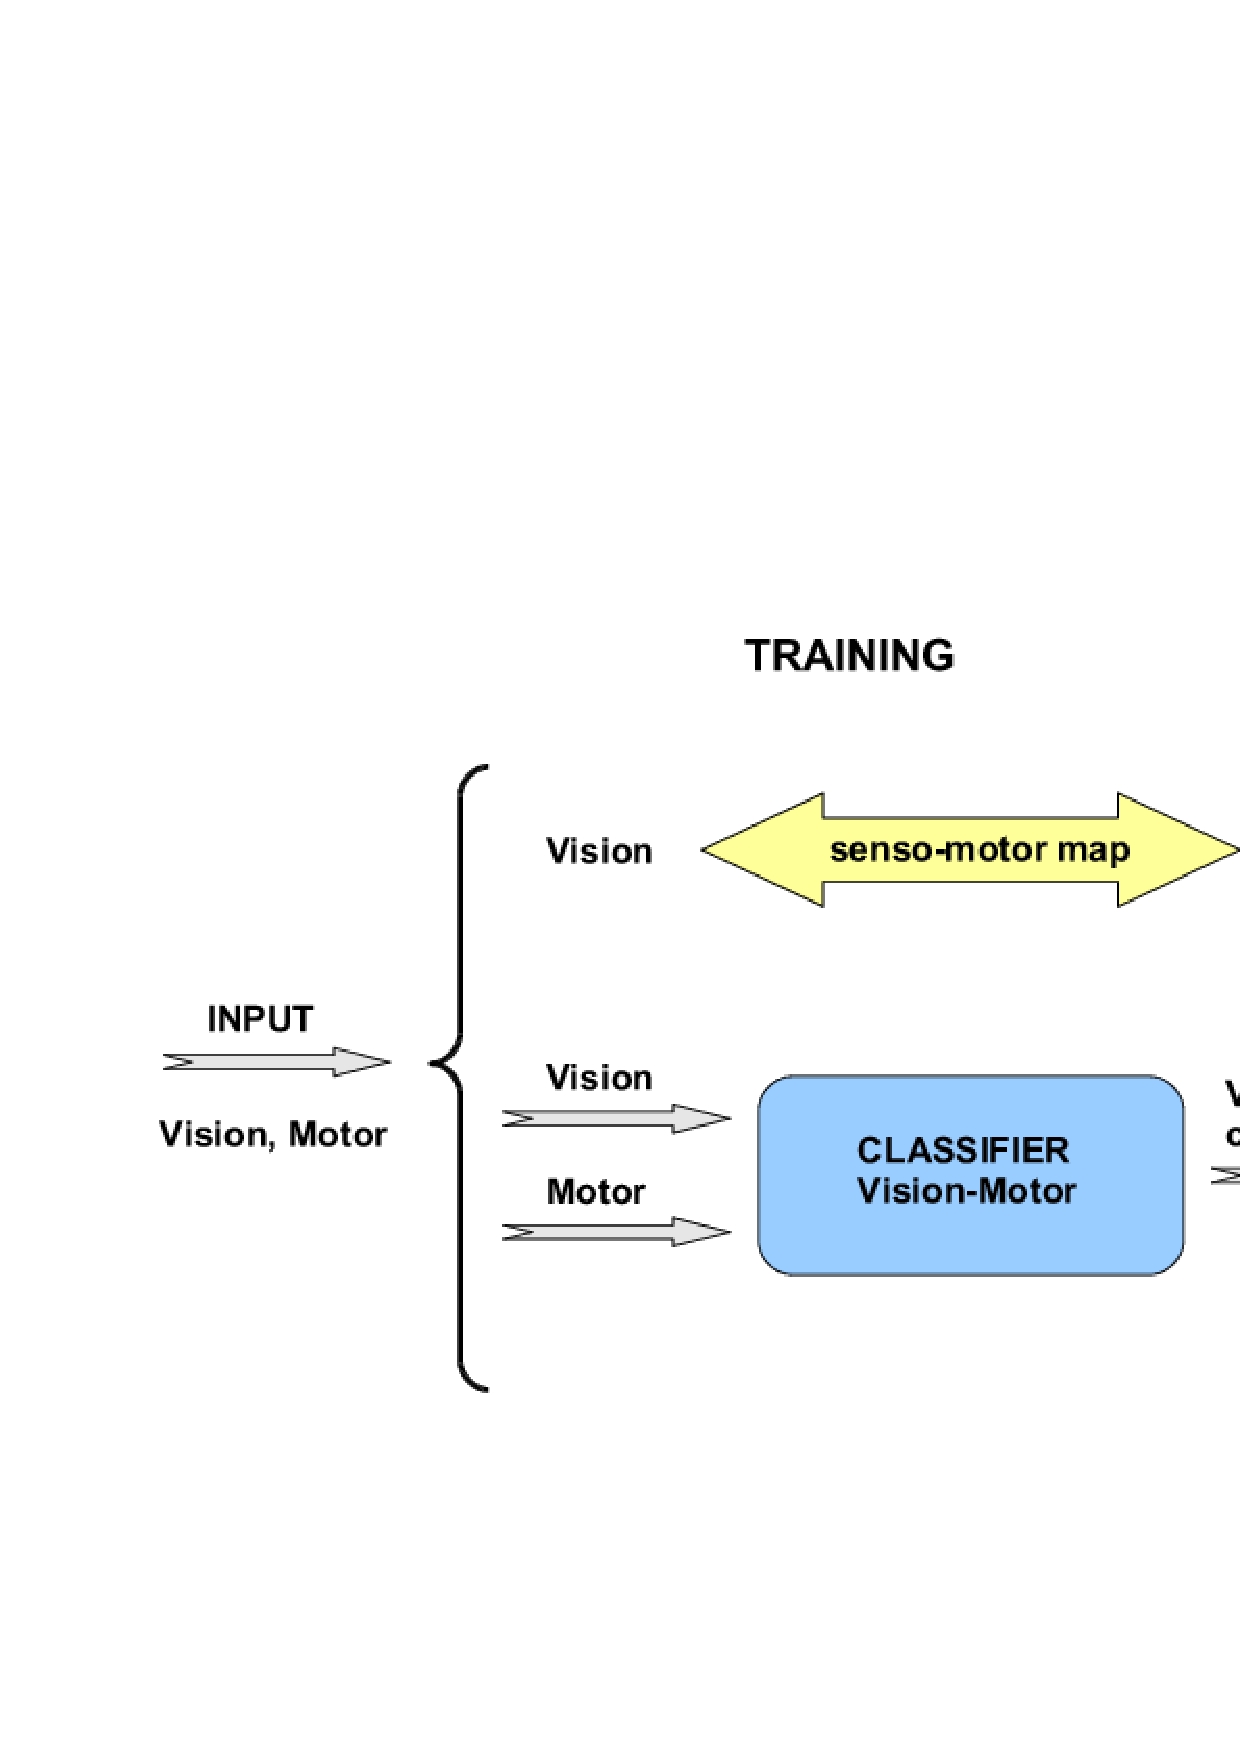
\includegraphics[width=0.7\textwidth]{images/train_fig}
	\caption{blabla}
	\label{fig:training-scheme}
\end{figure}

\begin{figure}[h!]
        \centering
        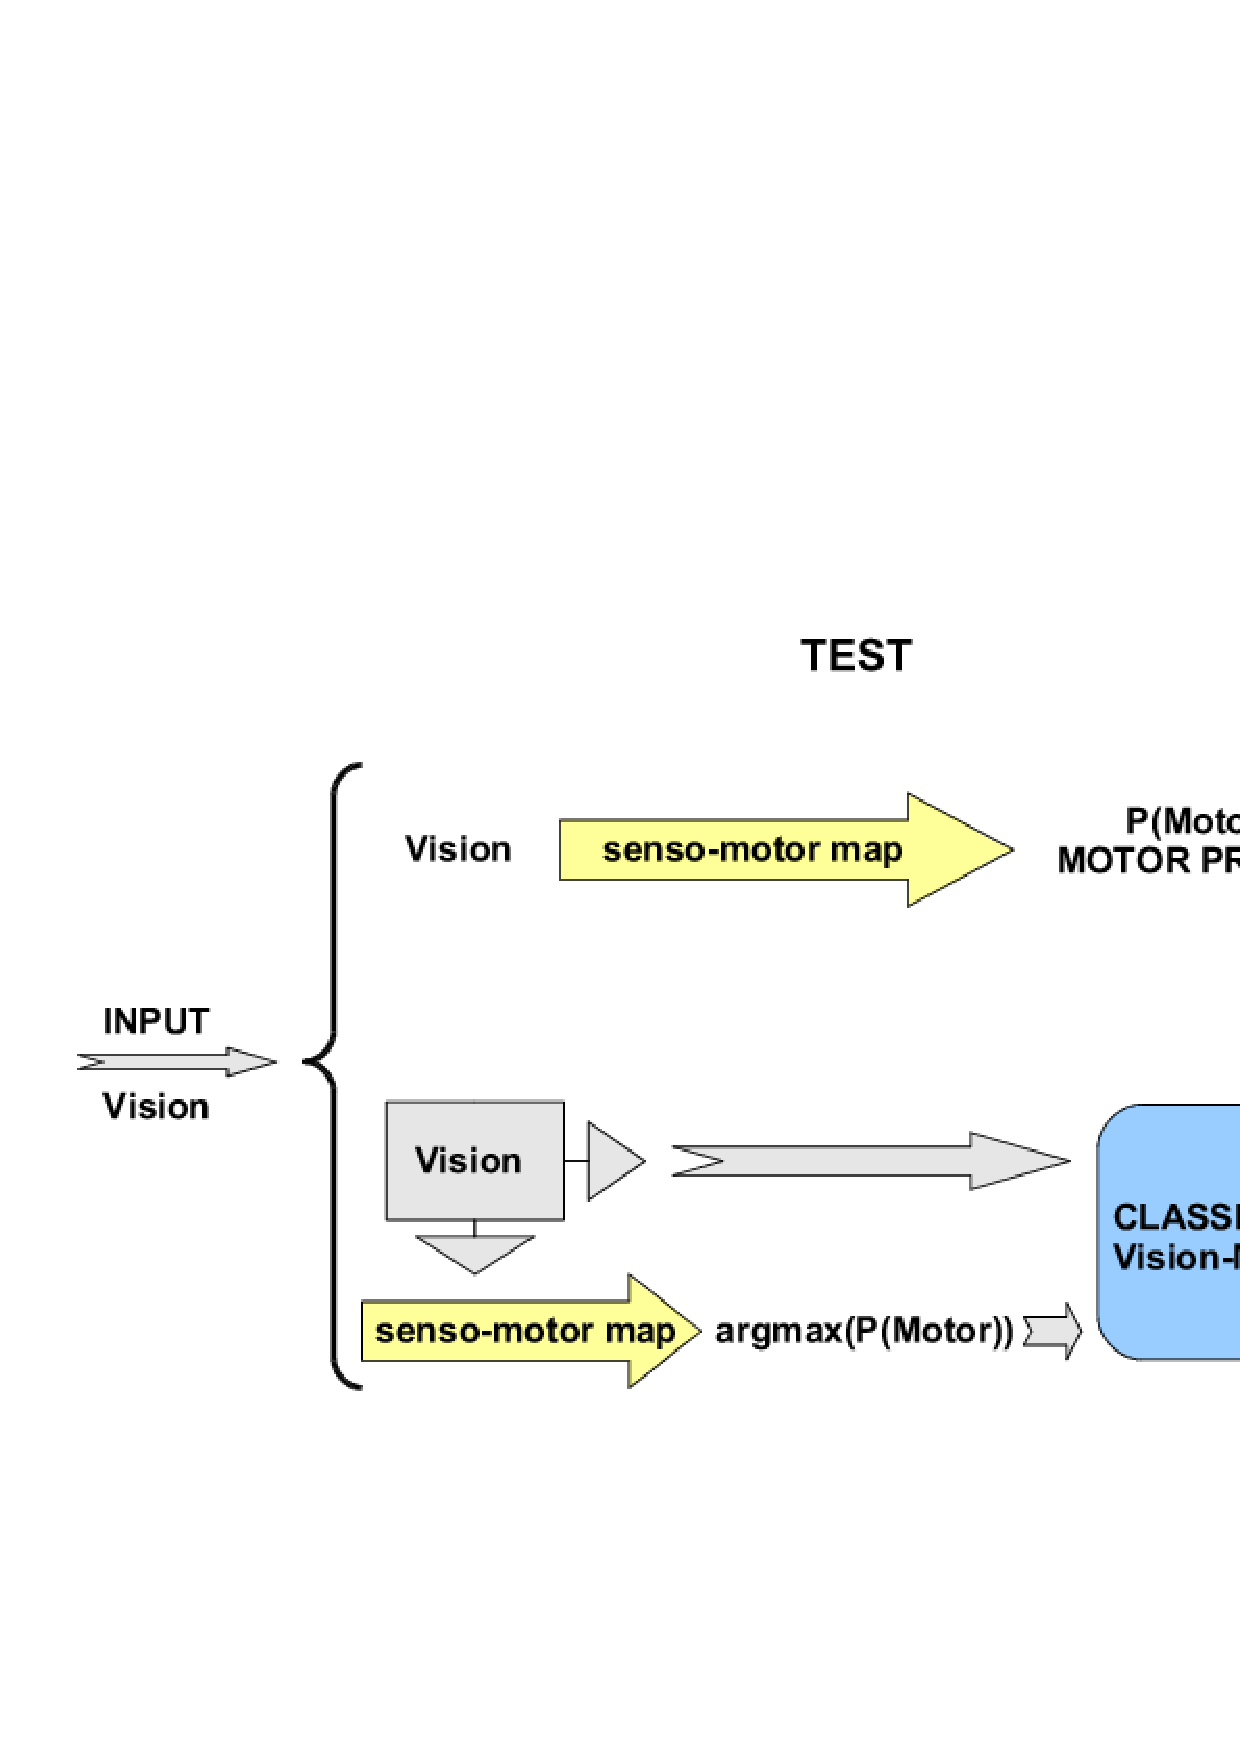
\includegraphics[width=0.7\textwidth]{images/test_fig}
        \caption{blabla}
        \label{fig:test-scheme}
\end{figure}


%\vskip -0.5cm

The training phase is schematically illustrated in Figure \ref{fig:training-scheme}. During training, the system receives as input labeled visual and motor
perceptual representation. These correspond to the seen object (Visual Perceptual Representation, VPR) and to the grasp posture of the hand
manipulating the object (Motor Perceptual Representation, MPR). On these data, the system builds in parallel two functions: a senso-motor map
between VPR and MPR (Figure \ref{fig:test-scheme}, top) and a classification function receiving as input both modalities, trained
to recognize the perceived object (Figure \ref{fig:training-scheme}, bottom). Technical details on how we compute the sensor motor map and the
multi-modal classifier are reported in section .. and ...

Figure \ref{fig:test-scheme} shows the test phase with its two possible outcomes. When receiving as input a VPR of a known object, the system can
opt for two different types of action:
\begin{itemize}
\item {\em Activation of the sensor-motor map}. This produces as an output an estimate of the most probable motor grasps associated 
to that object, with the corresponding 
MPRs for the grasp postures. We call this estimates {\em motor priming}, as they would correspond in an embodied agent to the pre-activation of the possible 
grasps. A detailed description of how we obtain the motor priming is given in section .....

\item {Object classification}. Note that, having learned the object on two modalities, the classifier needs as input a VPR and its corresponding MPR. We derive the
{\em not perceived} MPR using the senso-motor map (Figure \ref{fig:test-scheme}, bottom). The obtained motor priming is then given as input to the classifier with the VPR. We stress again that the clasifier recognizes the object on the basis of its visual appearance and of how it can be grasped. Experiments
reported in section ... shows clearly that this leads to a significant increase in performance compared to using only visual information.

\end{itemize}

{\bf FIXM EBABS; NICOLETTA; CLAUDIO: io metterei qui la descrizione delle visual and sensomotor features, senza farci una sezione specifica per ognuna}

\subsection{Perceptual representations}
\label{sec::vision}
\begin{figure}
	\centering
	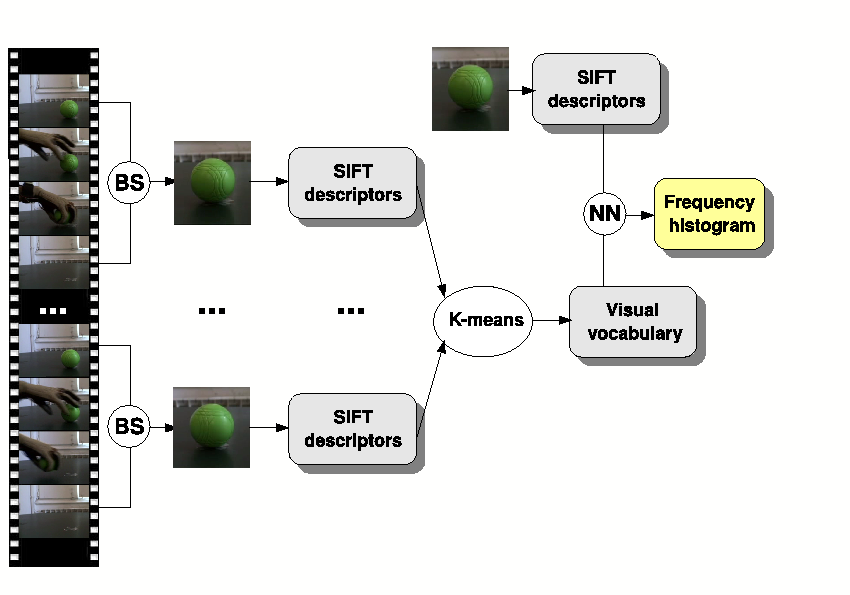
\includegraphics[width=0.8\textwidth]{images/schema_vision}
	\caption{A schema of the vision unit. First, suitable frames are extracted from the sequence and objects are located by means of background subtaction (BS). SIFT descriptors of a set of random points are input of a clustering step to get to the final visual vocabulary. Finally, each image is represented with respect to the vocabulary adopting a nearest neighbour (NN) strategy (see text for details).}
	\label{fig::vision}
\end{figure}

\section{Vision unit}
\label{sec::vision}
As we will discuss in Sec. \ref{sec::experiments}, the system gathers, as one input, a video sequence acting as {\it spectator}, whose focus is on object appearance. The goal of the vision unit is to process the signal to obtain a global model of a set of given objects.
Figure \ref{fig::vision} shows the pipeline of the vision unit when considering only one object (the same procedure is applied to the whole set of objects). Among the sequence, we first select the frames showing only the object  without any occlusion, then we locate more precisely its position by means of a simple background subtraction. 
Although in our application there is not an explicit object recognition step, it is clear from the architecture pipeline that a robust and specific object model is functional to subsequent analysis. It is worthwhile also to mention that with the terms {\it object recognition} we indicate the characterization of a specific object instance (againts the concept of categorizing classes of objects).
We adopt an approach based on local features to describe image structures: because of their popularity a rich variety of local measurements have been proposed in the literature \cite{harris,schmid,lowe} and applied successfully to objects recognition and categorization problems (see \cite{csurka,ferrari} just to name a few). 
Local approaches tipically include two distinct steps: keypoints extraction and description. 
However, in our case, a keypoint based-representation often ends up into a poor description
due to the limited size of the images. We thus built our representation by extracting enough 
random points  guaranteeing a more homogenous sampling.
We chose to adopt SIFT descriptors \cite{lowe,schmid2} to model image patches around these points, obtaining a set of {\it words} for each image.\\
To avoid redundancy and include some global information in our model, we apply k-means \cite{wong}, following the well-known bag-of-words approach \cite{csurka}. 
We thus build a {\it global} vocabulary, containing SIFT descriptions of all known objects. 
Image representation is obtained by means of frequency histogram of visual words, selecting for each random point extracted from the image 
the most similar visual word as nearest neighbor. A normalization step may be advisable for the subsequent data processing.
\subsection{Learning the Visuo-Motor Map}
\label{sec::regression}
\section{Regression model}
\label{sec::regression}

The mapping between object description and grasp description (Fig. \ref{fig::implementation})  corresponds to a vector-valued regression problem. 
Given a training set of input-output pairs $\{({\bf x}_i, {\bf y}_i): {\bf x}_i \in \rone^p,{\bf y}_i \in \rone^d \}_{i=1}^n$, 
the aim is to estimate a deterministic map from images of objects to sensor values able to generalize on new data. 
In other words, we want to estimate a function $\boldsymbol{f}:~\rone^p~\to~\rone^d$, 
where $p$ is the number of features representing the input images and $d$ is the number of sensors. This requires an estension of supervised learning methods to the vector valued setting.
Assuming that the data is sampled  {\em i.i.d.} on $\rone^p \times \rone^d$ according to an unknown probability 
distribution $P({\bf x}, {\bf y})$, ideally the best estimator minimizes the prediction error, measured by a loss function $V({\bf y},\boldsymbol{f}({\bf x}))$, on all possible examples. Since $P$ is unknown we can exploit the training data only. 
On the other hand, the minimization of the \emph{empirical risk}:  $
\mathcal{E}_n(\boldsymbol{f})=\frac{1}{n}\sum_{i=1}^{n} V({\bf y}_i,\boldsymbol{f}({\bf x}_i))$ leads to solving an ill-posed problem, since the solution is  not stable and achieves poor generalization. 
Regularized methods tackle the learning problem by finding the estimator that minimizes a functional composed of a data fit term and a penalty term, which is introduced to favour smoother solutions that do not overfit the training data. The use of kernel functions allows to work with non-linearity in a simple and principled way. In \cite{MicchPon05Onlearning} the vector-valued extension of the scalar Regularized Least Squares method was proposed, based on matrix-valued kernels that encode the similarities among the components $f^\ell$ of the vector-valued function $\boldsymbol{f}$.
In particular we consider the minimization of the functional: 
\begin{equation}
\frac{1}{n}\sum_{i=1}^{n} ||{\bf y}_i - \boldsymbol{f}({\bf x}_i)||_d^2 + \lambda ||\boldsymbol{f}||_K^2
\label{eq:Tikh}
\end{equation}
in a Reproducing Kernel Hilbert Space (RKHS) of vector valued functions, defined by a kernel function $K$.
The second term in (\ref{eq:Tikh}) represents the \emph{complexity} of the function $\boldsymbol{f}$ and the regularizing parameter $\lambda$ balances the amount of error we allow on the training data and the smoothness of the desired estimator. The representer theorem \cite{dev04representer,MicchPon05Onlearning} guarantees that the solution of (\ref{eq:Tikh}) can always be written as: $\boldsymbol{f}({\bf x}) = \sum_{i=1}^n K({\bf x}, {\bf x}_i){\bf c}_i,$ where the coefficients ${\bf c}_i$ depend on the data, on the kernel choice and on the regularization parameter $\lambda$. The minimization of (\ref{eq:Tikh}) is known as Regularized Least Squares (RLS) and consists in inverting a matrix of size $nd \times nd$.\\
Tikhonov Regularization is a specific instance of a larger class of regularized kernel methods
studied by \cite{LoGerfo08Spectral} in  the scalar case and extended to the vector case in [preprint].
These algorithms, collectively know  spectral regularization methods, provide a  computational alternative to Tikhonov regularization and are often easier to tune. In particular we consider 
iterative regularization methods with early stopping, where the role of the regularization 
parameter is played by the number of iteration. Besides Tikhonov regularization, in  the experiments we consider L2 boosting (Landweber iteration) \cite{bulmann02boosting,LoGerfo08Spectral} and the $\nu$-method \cite{LoGerfo08Spectral}. 
%
%An alternative approach to find a good estimator $\boldsymbol{f}$ is to proceed by means of iterative algorithms. 
%These methods iteratively minimize the empirical risk and are regularized by 
%stopping the iterations before reaching convergence \cite{Yao07Early}.
%The main idea is to start with an approximate
%solution and iteratively add a correction in the direction
%opposite to the gradient of the empirical risk.
%By early stopping the procedure, a regularized solution is achieved, hence avoiding overfitting.
%The number of iterations $m$ plays the role of the regularization parameter $\lambda$.
%When computing the solution for a specific number of iterations, 
%the process yields the solutions for all the previous steps, therefore it
%is computationally inexpensive to select the optimal stopping point.
%For the experiments we will consider only the Landweber \cite{bulmann02boosting} and the $\nu$-method \cite{LoGerfo08Spectral}.

% Standard regression techniques start with a parametric representation of the desired map and estimate its parameters by minimizing the prediction error on the training data, the so called empirical risk. These methods, apart from imposing a predefinite shape of the estimator, are known to overfit, that is they rely too much on the training data, which usually is affected by an unknown amount of noise. Regularized techniques introduce a penalty term on the complexity of the estimator, favouring smoother solutions that do not overfit the training data.
%We now briefly introduce some mathematical notation to better describe these methods. 
% The best possible estimator is the one minimizing the expected risk:
% $$
% I[f] \equiv  \int_{\rone^p \times \rone}~V(y, f({\bf x})) P({\bf x}, y)~d{\bf x}dy,
% $$
% where $V(y,f({\bf x}))$ is the loss function measuring the error of
% predicting $y$ by $f({\bf x})$ and in our case we chose to work with the square loss $(y-f(x))^2$.
%Ideally the best estimator minimizes the prediction error, measured by a loss function $V({\bf y},\boldsymbol{f}({\bf x}))$, on all possible examples, but since $P$ is unknown we can exploit the training data only. On the other hand, the minimization of the \emph{empirical risk}:  $
%\mathcal{E}_n(\boldsymbol{f})=\frac{1}{n}\sum_{i=1}^{n} V({\bf y}_i,\boldsymbol{f}({\bf x}_i))$ leads to solving an ill-posed problem, since the solution is not unique, not stable and
%with poor generalization properties. 

\subsection{Learning the Visuo-Motor Classifier}
%\subsection{Building the visuo-motor classifier}
\label{sec::classifier}
FIXME TATI, BABS

%\subsection{Multi-modal object recognition}
%\label{sec::recognition}
%Lastly, all ideas detailed above can be put together. In the testing
phase, when only visual features are available, our system performs three steps:

\begin{enumerate}

  \item the VPR is extracted from the visual appearance of the object. Based upon
    it, the label of the object is predicted;
  \item this label is used to choose the appropriate VMM;
  \item the VMM reconstructs the grasp associated with the object and this
    MPR is then used, alone or joined with the VPR, to recognize the object.

\end{enumerate}

\textbf{CC: non so di quanto aiuto possa essere qui. la struttura e`, ora come ora,
un po' traballante perche' manca uno schema generale ben fatto. manca completamente
questo passo che determina quale VMM utilizzare. io quest'ultima sottosezione forse
la eliminerei del tutto.}


\section{Experimental results}
\label{sec::experiments}
This section reports the experimental validation of our model.
We begin by 
testing the model on real data (section \ref{res:real}), showing that
by joint modeling visual and motor information it is possible to
achieve a significant boost in recognition, compared to using visual
information only. 
We proceed evaluating the quality of the reconstructed archetypal grasp via regression
(section \ref{res:regression}).
We then show that, whenever the motor information
is not perceived by the agent, it is still possible to get a better performance
by using our VMM to generate an archetypal grasp as input for the classifier
(section \ref{res:reconstruct}).



%The visual / motor grasping data used to build the VMM is contained in
%the CONTACT Visuo-Motor Grasping dataBase (VMGdB). The VMGdB is obtained
%by having $20$ subjects repeatedly grasp $7$ objects in $5$ different ways;
%meanwhile, two Watec \emph{WAT-202D} colour cameras and a $22$-sensors
%Immersion \emph{CyberGlove} \cite{cyberglove} right-hand sided dataglove
%were used to obtain a fair visual / motor representation of the grasping acts.
%Absoute timestamps are used to synchronise the video and numerical streams.
%In this setting we only used one of the cameras, focussed on the object and
%lateral to the subject; the dataglove provides $22$ $8$-bit numbers
%linearly related to the angles of the subject's hand joints.

%The VMGdB purposedly enforces no control over the illumination of the set-up,
%nor any guarantee on the colours of objects or of the background; moreover,
%each object has been grasped in several different ways, and the same grasp
%has been used for several different objects. This makes the VMGdB
%a realistic representation of the act of grasping an object.


\subsection{Results with real motor data}
\label{res:real}

The first set of experiments was conducted on real data, namely motor data
registered by the users when grasping the objects, and the corresponding images.
Our goal here was to show the advantage in recognition achieved by modelling the object
on both modalities, and at the same time compare the three possible joint
modelling strategies presented in section \ref{sec::classifier}, to chose the best one.

Experiments were performed considering the whole set
of 5200 data and choosing randomly 130 samples for
training and 2600 samples for testing. The random extraction was repeated
defining 10 different splits and the classification was executed using SVM,
one-vs-all multiclass extension. We used the Gaussian Kernel for the
visual and motor modalities, both when considered separately and in the
integration approach (two Gaussian Kernels combined in MCK). The best
learning parameters were selected through cross validation.

% \begin{table*}[tbp]
% \centering \footnotesize
% \begin{tabular}{c|@{}c@{}|@{}c@{}|@{}c@{}|@{}c@{}|@{}c@{}|@{}c@{}|@{}c@{}|@{}c@{}|@{}c@{}|@{}c@{}|@{}c@{}|@{}c@{}|@{}c@{}|@{}c@{}|@{}c@{}|@{}c@{}|@{}c@{}|@{}c@{}|@{}c@{}|@{}c@{}|@{}c@{}|@{}c@{}|@{}c@{}|}
%   \cline{2-8} \cline{10-16} \cline{18-24}
%   % after \\: \hline or \cline{col1-col2} \cline{col3-col4} ...
% \multirow{7}{*}{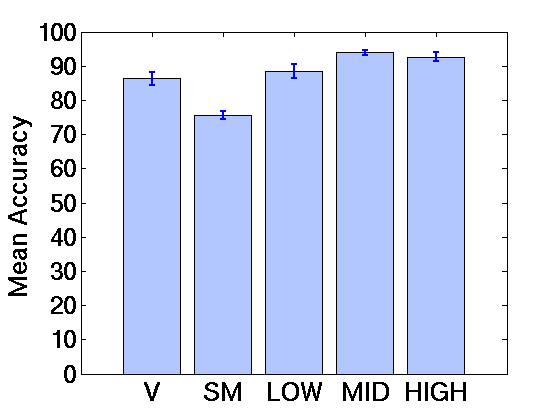
\includegraphics[width=0.18\textwidth]{images/real}}& 88.6&	0.9&	1.4&	1.0&	7.2&	0.4&	0.5&&	77.2&	0.3&	0.3&	0.7&	0.4&	19.9&	1.2&&	96.5&	0.1&	0.0&	0.9&	1.2&	1.2&	0.2\\
%   \cline{2-8} \cline{10-16} \cline{18-24}
% &0.1&	80.9&	0.1&	0.3&	16.5&	0.0&	2.2&&	1.1&	58.9&	25.3&	1.2&	2.0&	9.5&	2.1&&	0.0&	91.8&	2.5&	1.1&	2.8&	1.4&	0.5\\
%   \cline{2-8} \cline{10-16} \cline{18-24}
% &3.4&	0.2&	88.3&	0.3&	4.3&	2.8&	0.6&&	0.5&	5.7&	79.0&	0.5&	0.9&	8.6&	4.9&&	0.1&	1.8&	94.4&	0.1&	0.3&	2.5&	0.8\\
%   \cline{2-8} \cline{10-16} \cline{18-24}
% &0.0&	0.0&	0.4&	75.1&	24.5&	0.0&	0.0&&	2.6&	0.6&	0.2&	96.6&	0.0&	0.2&	0.0&&	0.0&	0.0&	0.0&	100.0&	0.0&	0.0&	0.0\\
%   \cline{2-8} \cline{10-16} \cline{18-24}
% &0.7&	1.6&	1.9&	1.3&	90.4&	1.6&	2.7&&	0.0&	0.8&	0.5&	0.0&	77.7&	0.3&	20.9&&	0.0&	0.1&	0.0&	0.1&	88.4&	0.0&	11.4\\
%   \cline{2-8} \cline{10-16} \cline{18-24}
% &0.0&	0.0&	0.0&	0.1&	1.8&	98.1&	0.0&&	13.0&	1.7&	6.8&	0.3&	0.9&	70.7&	6.7&&	0.7&	0.2&	0.2&	0.1&	0.6&	98.0&	0.2\\
%   \cline{2-8} \cline{10-16} \cline{18-24}
% &2.2&	2.4&	3.1&	1.2&	7.1&	0.9&	83.2&&	0.3&	4.8&	1.2&	0.8&	17.9&	6.3&	68.7&&	0.4&	2.0&	0.2&	0.4&	7.2&	1.4&	88.5\\
%   \cline{2-8} \cline{10-16} \cline{18-24}
% \multicolumn{1}{c}{} &\multicolumn{7}{c}{} &\multicolumn{1}{c}{}& \multicolumn{7}{c}{} &\multicolumn{1}{c}{}& \multicolumn{7}{c}{}\\
% \multicolumn{1}{c}{\normalsize(a)} &\multicolumn{7}{c}{\normalsize(b)} &\multicolumn{1}{c}{}& \multicolumn{7}{c}{\normalsize(c)} &\multicolumn{1}{c}{}& \multicolumn{7}{c}{\normalsize(d)}\\
% \end{tabular}
% \caption{}
% \label{table1}
% \end{table*}

\begin{figure*} \centering
  \begin{tabular}{@{}c@{}@{}c@{}@{}c@{}}
    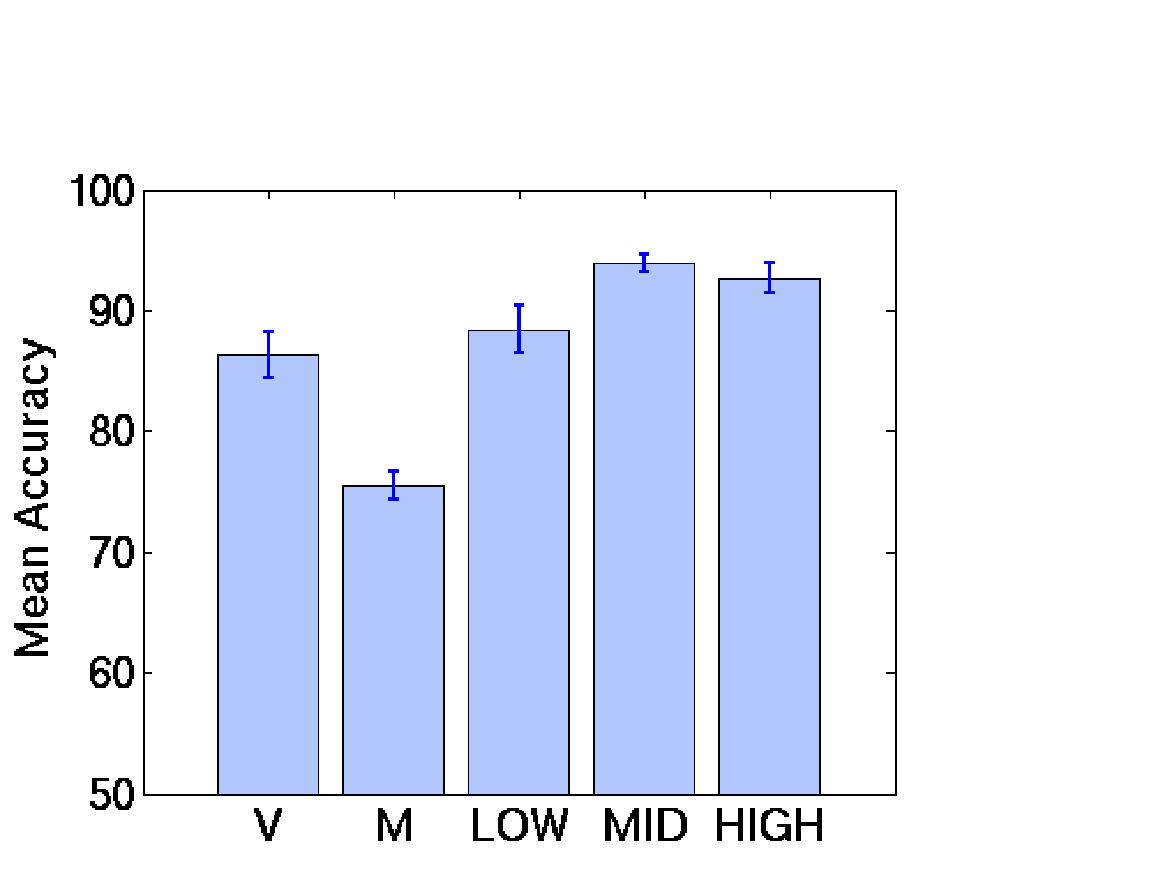
\includegraphics[width=0.25\textwidth]{images/real_.pdf} &
    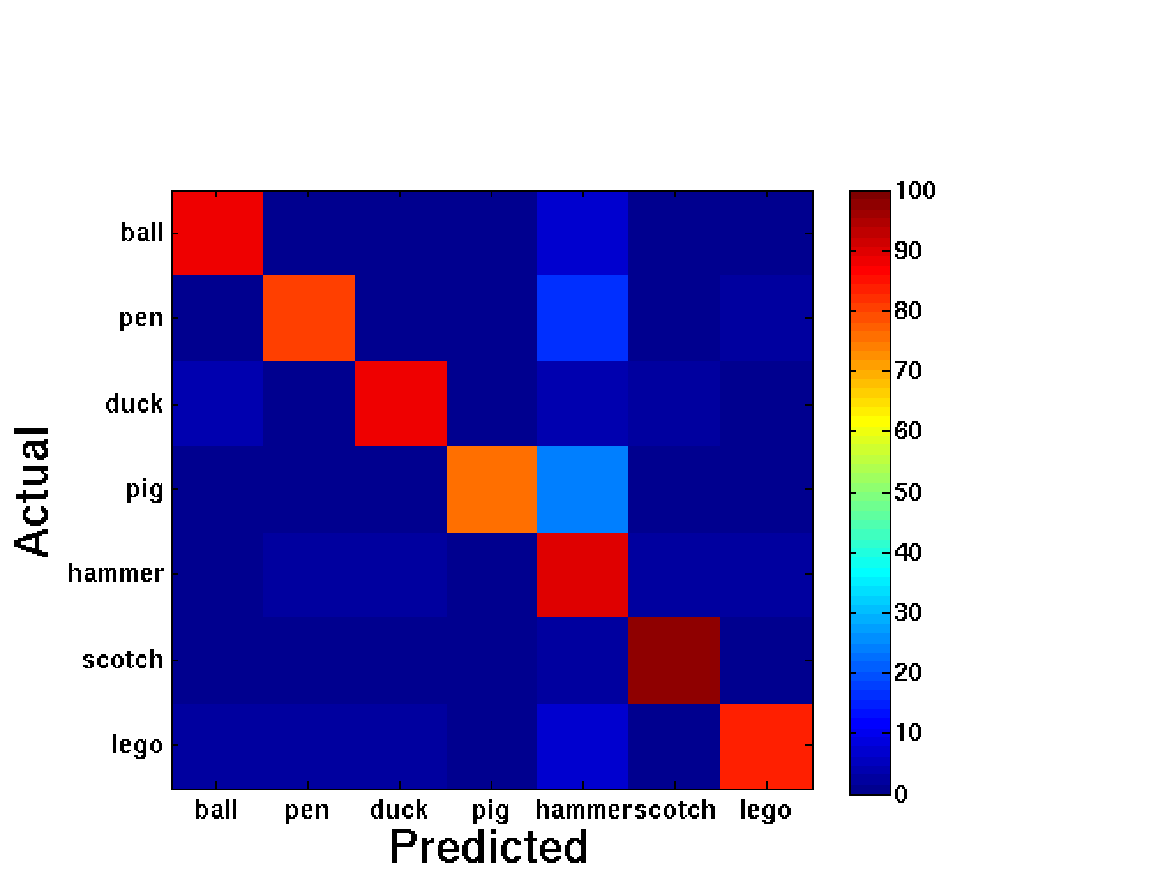
\includegraphics[width=0.25\textwidth]{images/conf_vis.pdf} &
    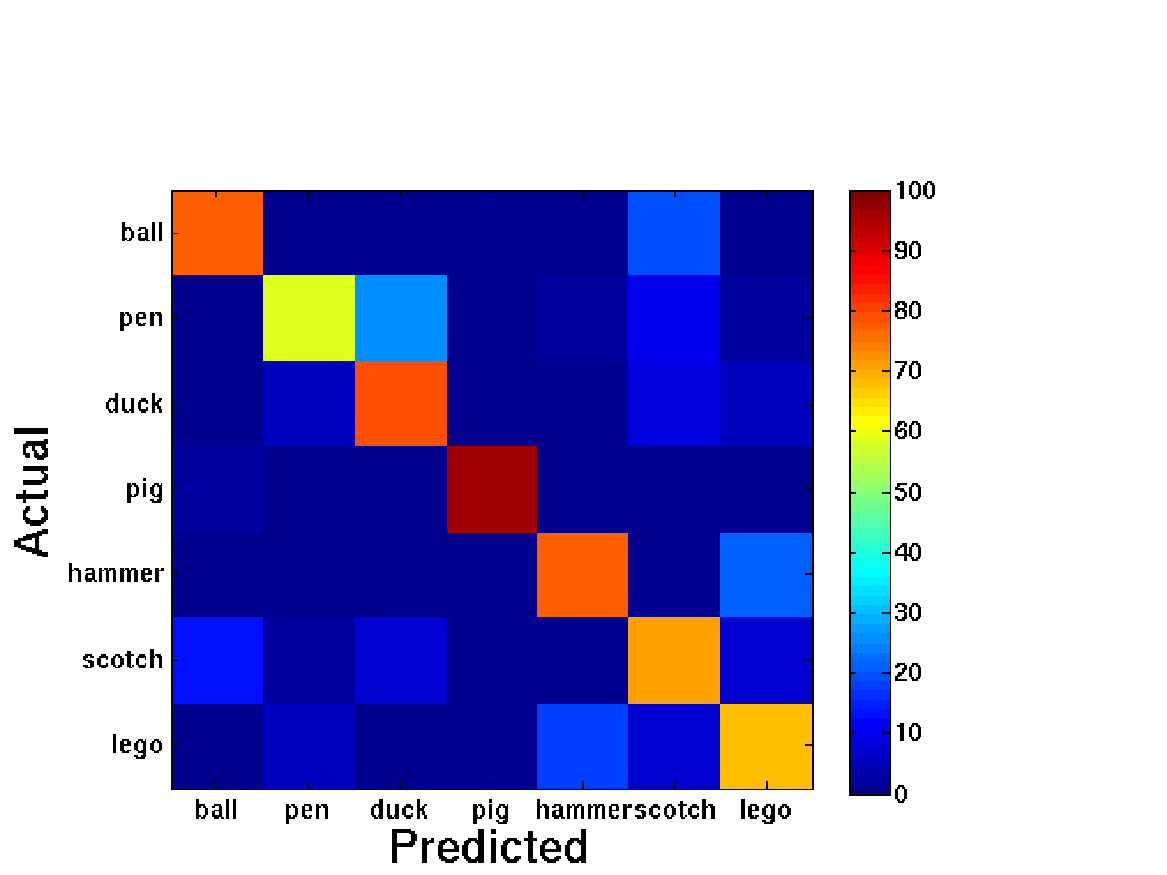
\includegraphics[width=0.25\textwidth]{images/conf_mot.pdf} \\
(a) & (b) & (c)\\
    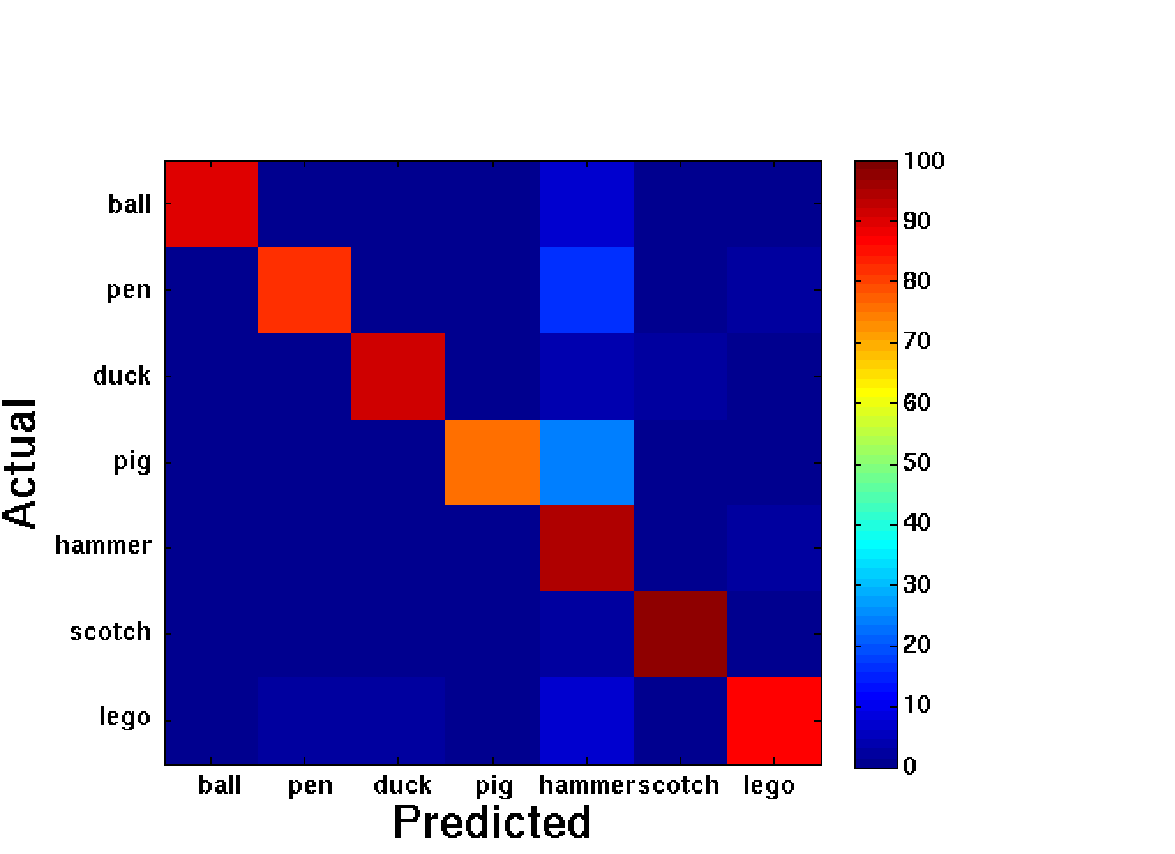
\includegraphics[width=0.25\textwidth]{images/conf_low_real.pdf} &
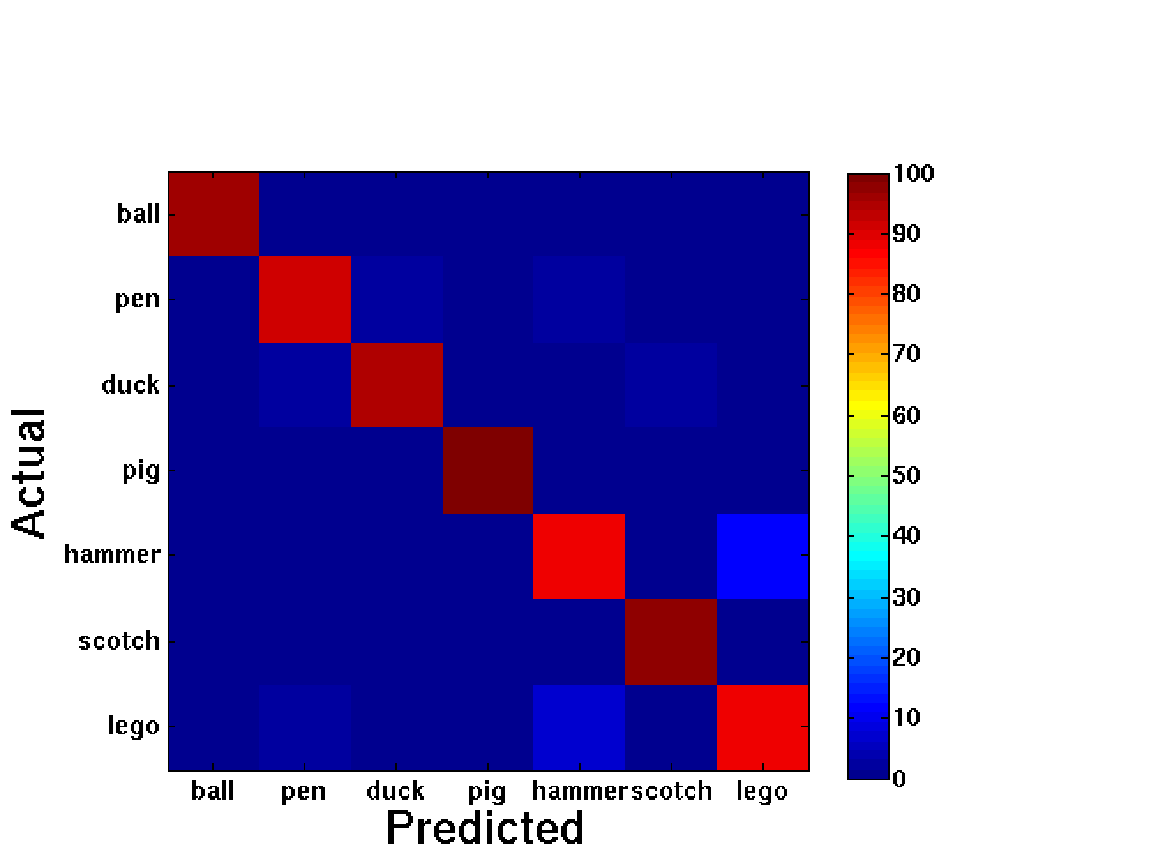
\includegraphics[width=0.25\textwidth]{images/conf_mck_real.pdf} &
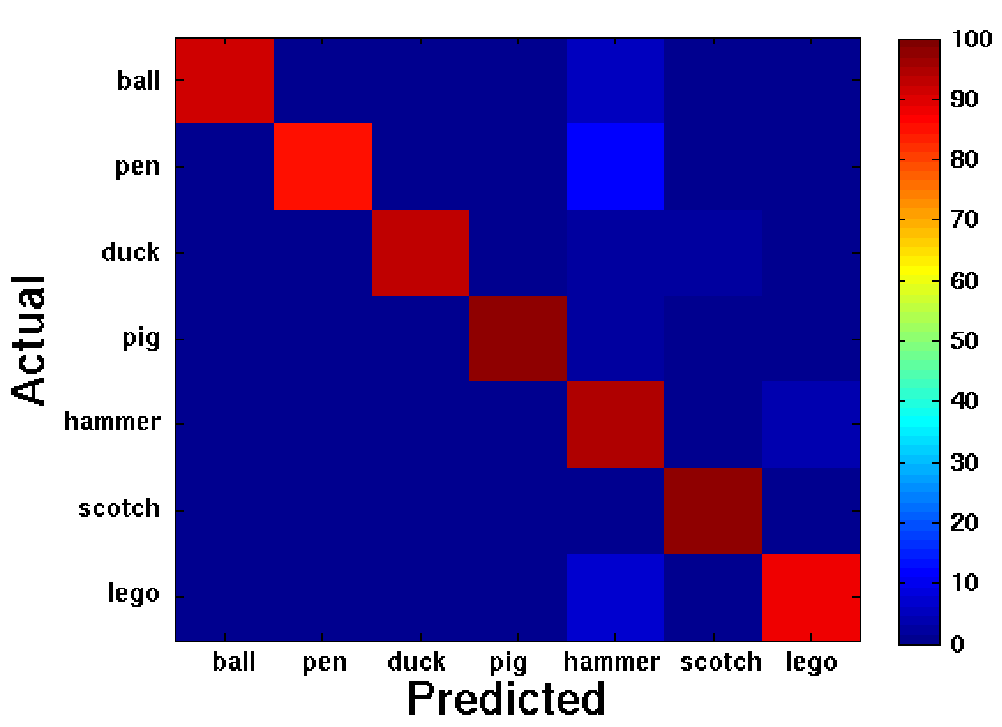
\includegraphics[width=0.25\textwidth]{images/conf_das_real.pdf} \\
    (d) & (e) & (f)\\
  \end{tabular}
  \caption{(a) Classification mean accuracy of the seven objects averaged
    on the ten splits; (b) confusion matrix using visual features; (c) confusion
    matrix using motor features; (d) confusion matrix using the low level
    feature integration; (e) confusion matrix using the mid level
    feature integration; (f) confusion matrix using the high level
    feature integration.}
  \label{fig:real_data}
\end{figure*}

Figure \ref{fig:real_data}-a shows the overall recognition results obtained by using only visual
information (V), only motor information (M), or the two combined together, with the three proposed approaches (LOW, MID, HIGH). We see in general that using the visual information we obtain better average performance ($86.37\%\pm1.91\%$) than using the motor one
($75.53\%\pm1.22\%$), and that their integration is clearly beneficial. The mid-level integration produces the best result ($93.94\%\pm0.77\%$): the gain in accuracy between MCK and only using visual features is $7.57\%$ (difference in accuracy
evaluated per split and then averaged on the 10 splits).
The second best result is obtained by using DAS ($92.65\%\pm 1.22\%$); we see that the difference in performance between DAS and MCK is 
not statistically significant, and therefore both are suitable candidates for the VMC module. 


Figure \ref{fig:real_data}-b, -f 
shows the confusion matrices obtained by the vision only classifier (Figure  \ref{fig:real_data}-b), by the 
motor only classifier (Figure \ref{fig:real_data}-c) and by the 
three integration methods: low-level (Figure \ref{fig:real_data}-d),
MCK  (Figure \ref{fig:real_data}-e)
and DAS (Figure \ref{fig:real_data}-f). 
It is clear that the combination of the two modalities leads to considerable 
advantages in the recognition of each object, for all methods. 
Consider for instance  the objects ``ball'' and ``pig'':  the mean accuracy is
respectively $88.6\%$ and $75.1\%$ using visual features and $77.2\%$ and $96.6\%$ using motor information. 
The ball was grasped in two different ways (with a `tripodal'' and a ``spherical'' grasp)
while the pig was manipulated only with the ``cylindric'' grasp, which was used just for this object.  
Thus, the grasp information is object-specific for the pig.
This led to an impressive increase in performance when using MCK, as we achieved a 100\% classification rate. Using
visuo-motor information is beneficial also for the ball, for which we obtained a multi modal recognition rate of 96.5\%.
Analogous considerations can be done for the two other approaches, and are omitted here for space reasons.

%For the
%``pen'', the ``tripodal'' and the ``spherical'' grasps were registerd while the ``pig'' was manipulated only with the ``cylindric'' grasp, which was used just for this object.  Thus, the grasp information is object-specific for
%the ``pig'' and this led to a good performance when using the motor data in object classification. With MCK we obtain respectively $96.5\%$ and $100.0\%$ for the ``pen'' and the ``pig''. 


From these experiments we can conclude that: (a) using a joint visual and motor object model leads to a very concrete 
advantage in performance during recognition, and (b) the MCK algorithm seems the most suitable for the joint 
modelling of the two modalities.

\subsection{Evaluation of reconstructed data}
\label{res:regression}
We now turn to the evaluation of the archetypal grasps generated by the VMM. We learn a neural network for each object seen during training; this results here in seven specific VMMs. If an object can be grasped in
only one way, the reconstructed motor data correspond to an estimate of this
grasp type. If the possible grasps are more than one, the reconstructed motor data
represent an estimate of the ``average'' grasp for that object.

To evaluate the goodness of the VMM in producing ``archetypal grasps'', we performed the following experiment:
 we divided the whole
dataset in two halves (2600 data each), using one for training and the other for testing. Specifically
we used the samples to:
\begin{enumerate}

  \item [(a)] Train the neural networks and predict the motor feature vectors of the
    testing set, for each
VMM associated to its specific object.	
 %using the correct object label for each. In this way we eliminate the uncertanity
 %   on which neural network should be used and evaluate the reconstructed sensorimotor vectors
 %   classifying them in terms of grasps.

  \item[(b)] Train a ``grasp classifier'' on the real motor information. The testing phase consisted
    in predicting the grasp label of the reconstructed motor vectors obtained from (a).
    We counted as  an error every time the predicted grasp was not one of the possible grasps
    associated with the relative object.

\end{enumerate}

We run the experiment on 10 splits of the whole dataset and we obtained an average error rate of
10.7\%. This is significantly low with respect to a random grasp labelling (error rate of 63\%).
We can conclude that the reconstructed grasp information is coherent with the real one, and therefore we expect 
that the archetypal grasp will turn out to be an informative feature when used for classification. 



%The most frequent case is of course that of an agent seeing an object without grasping it. 
%In that case, we propose an approach which still permits to take advantage from the VMM
%learned during training. More in detail:

%\noindent\textbf{Training}:  we consider a neural network for each object in
%the training phase resulting in 7 specific VMMs. If an object can be grasped in
%only one way, the reconstructed motor data correspond to an estimate of this 
%grasp type. If the possible grasps are more than one, the reconstructed motor data
%represent an estimate of the ``average'' grasp for that object.
%
%\noindent\textbf{Testing}: our system performs three steps:
%\begin{enumerate}
%  \item the VPR is extracted from the visual appearance of the object. Based upon
%    it, the label of the object is predicted;
%  \item this label is used to choose the appropriate VMM;
%  \item the VMM reconstructs the grasp associated with the object and this
%    MPR is then used, alone or joined with the VPR, to recognize the object.
%\end{enumerate}
%
%
%To begin with, it is important to evaluate the goodness of the VMM in producing ``archetipal grasps''.
%This means isolating the VMM performance not considering the object guessing
%in the first step of the recognition strategy in the test phase. To this end we divided the whole 
%dataset in two halves (2600 data each) using one for training and the other for testing. Specifically 
%we used the samples to:
%
%\begin{enumerate}
%
%  \item [(a)] train the neural networks and predict the sensorimotor feature vectors of the 
%    testing set using the correct object label for each. In this way we eliminate the uncertanity 
%    on which neural network should be used and evaluate the reconstructed sensorimotor vectors
%    classifying them in terms of grasps.
%
%  \item[(b)] train a ``grasp classifier'' on the real motor information, the testing phase consisted 
%    in predicting the grasp label of the reconstructed sensorimotor vectors obtained from (a). 
%    We considered an error each time the predicted grasp is not one of the possible grasps 
%    associated with the seen object. 
%
%\end{enumerate}
%
%We run the experiment on 10 splits of the whole dataset and we obtained an average error rate of
%10.7\% which is significativly low respect to a random grasp labelling (error rate of 63\%).
%This tells us that the reconstructed grasp information is coherent with the real one.
%

\subsection{Results with reconstructed data}
\label{res:reconstruct}


The most frequent case is of course that of an agent seeing an object without grasping it. 
In that case, our approach  still permits to take advantage of the VMC, using as 
motor input the archetypal grasp generated by the VMM.
More in detail, the system 
performs three steps (see Figure \ref{fig::reconstructed-schema} for a schematic representation):
\begin{enumerate}
  \item We extract the visual features  from the object's view. Based upon
    it, we generate an hypothesis on %predict 
	the label of the object using only visual data. 
%with a vision-only classifier;
  \item The hypothesis is used to choose the appropriate VMM.
  \item The VMM reconstructs the grasp associated with the object. This
    motor feature is then used, alone or jointly with the visual feature, to recognize the object.
\end{enumerate}
We evaluated this strategy by repeating the experiments described in Section \ref{res:real}, using as input only visual data.
For the implementation of the first step described above, we used the vision only classifier trained on real data
(see Section \ref{res:real}).


\begin{figure}
        \centering
        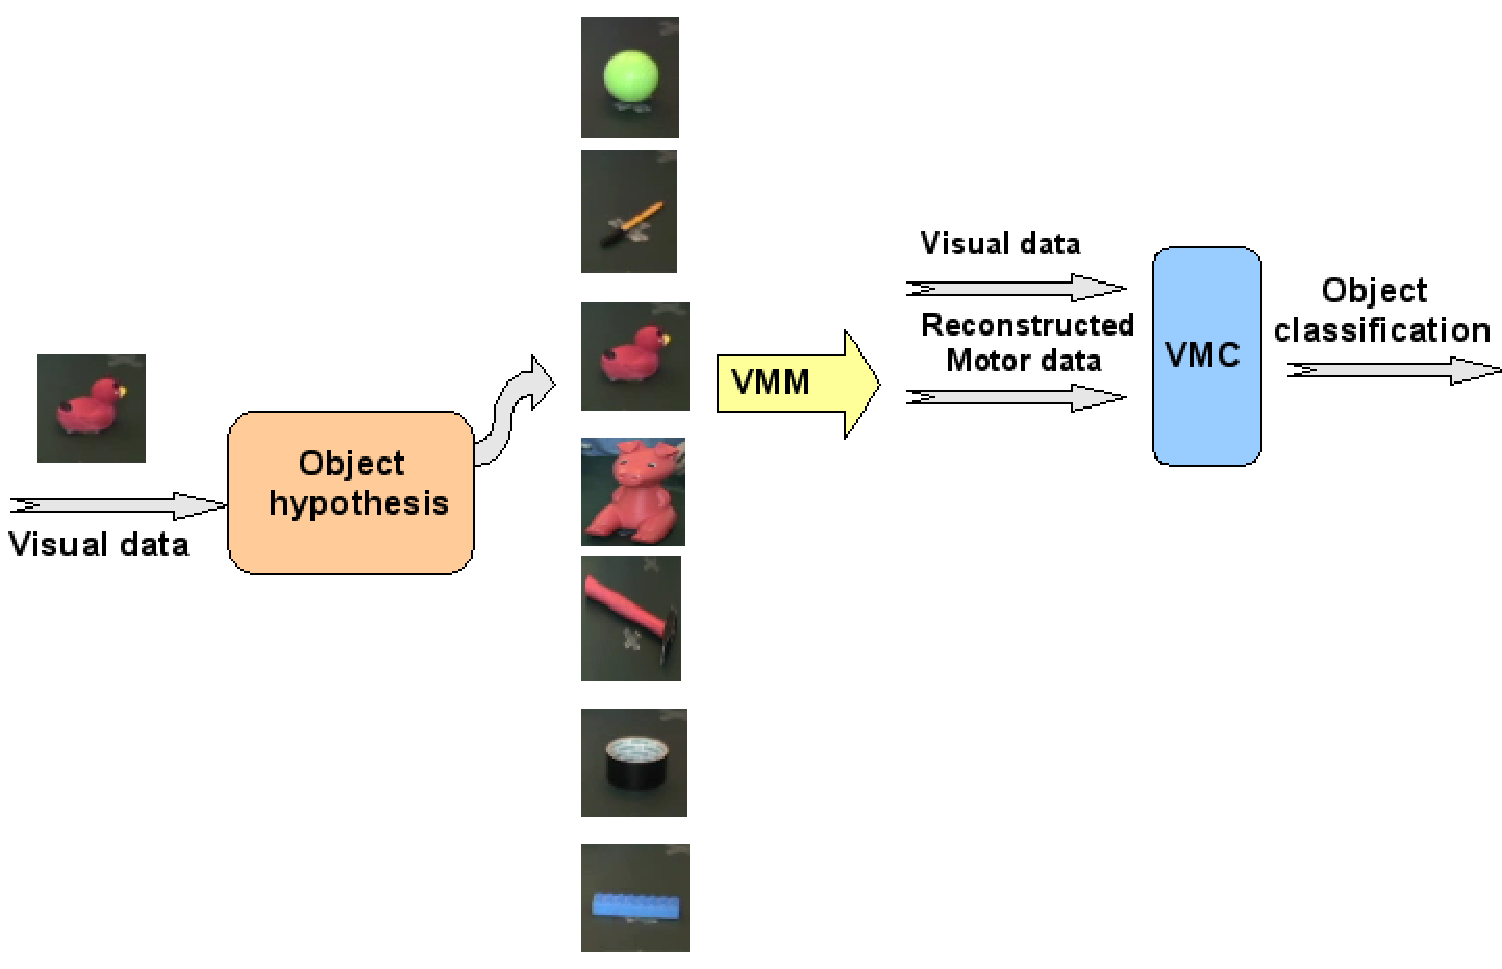
\includegraphics[width=0.5\textwidth]{images/schema_process.pdf}
        \caption{A schematic representation of how the reconstructed motor features are used in the VMC.}
        \label{fig::reconstructed-schema}
\end{figure}



 
%We repeated the classification experiments described in section \ref{res:real}, using as input only visual data. 
%We considered all the three steps defined in section \ref{res:regression}, using for the first one 
%the classifier on visual information (V) obtained from the set of
%experiments on real data.

\begin{figure*} \centering
  \begin{tabular}{@{}c@{}@{}c@{}@{}c@{}}
    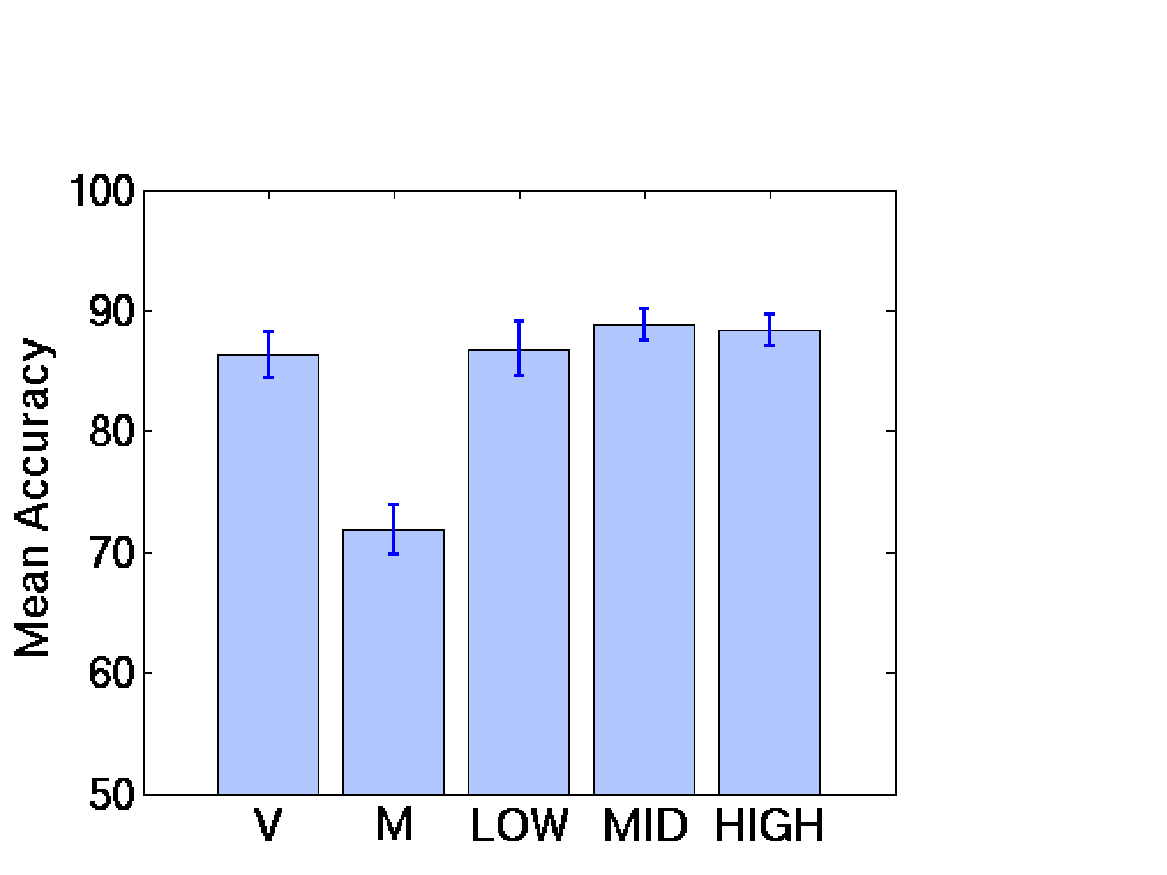
\includegraphics[width=0.25\textwidth]{images/ric_.pdf} &
    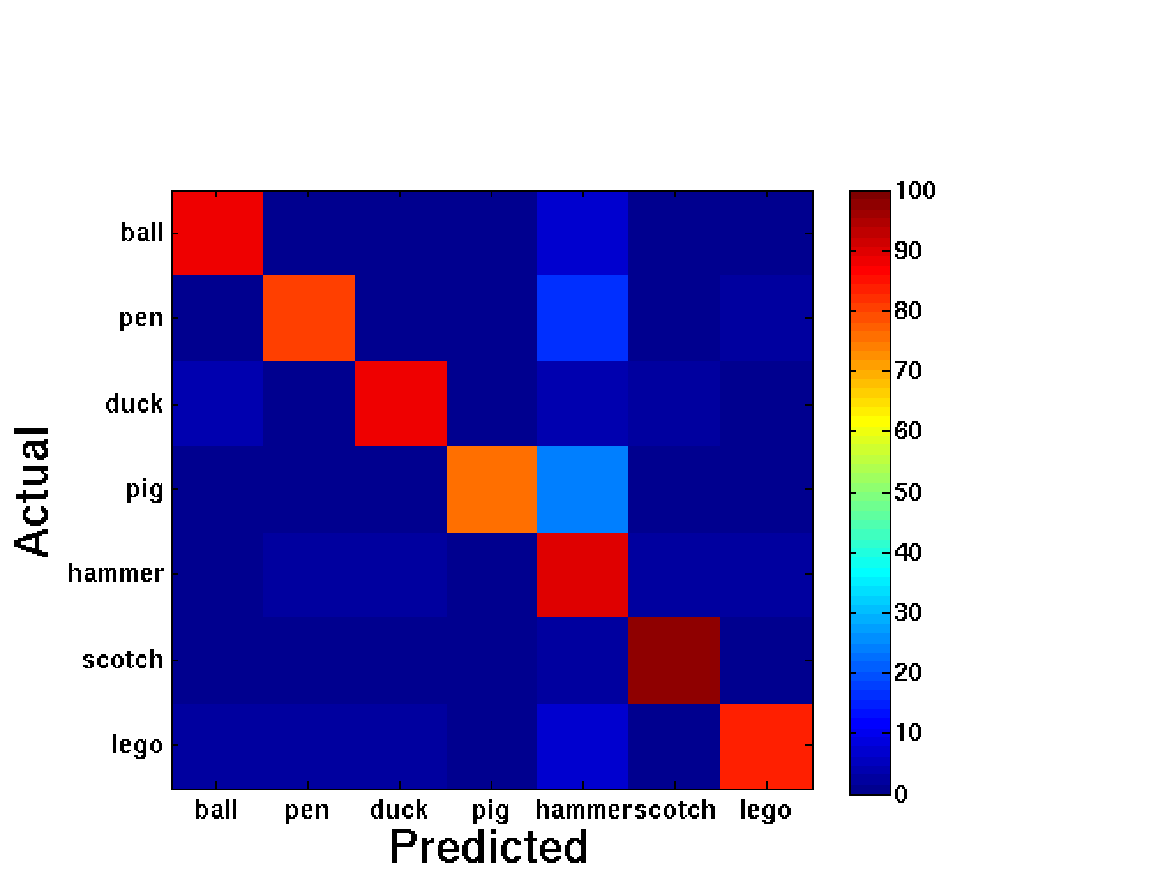
\includegraphics[width=0.25\textwidth]{images/conf_vis.pdf} &
    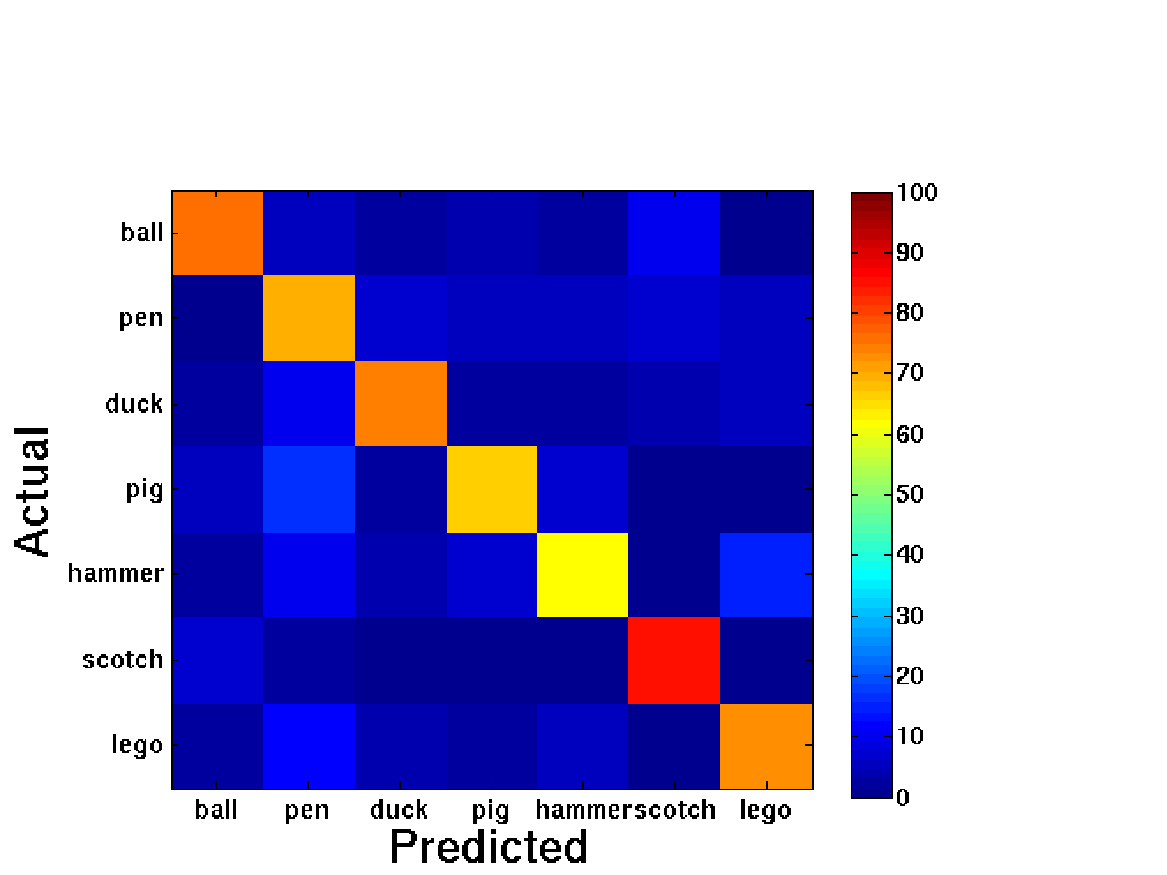
\includegraphics[width=0.25\textwidth]{images/conf_mot_ric.pdf} \\
(a) & (b) & (c)\\
    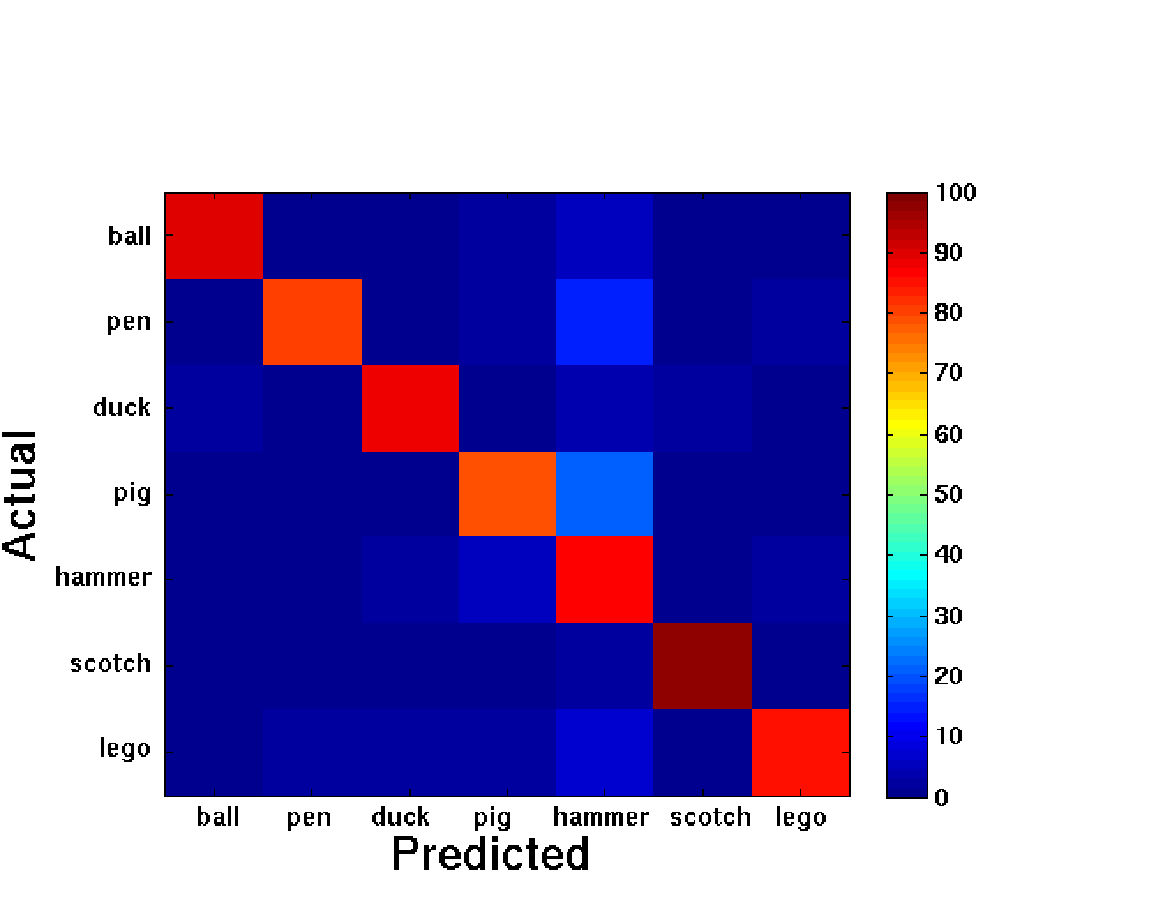
\includegraphics[width=0.25\textwidth]{images/conf_low_ric.pdf} &
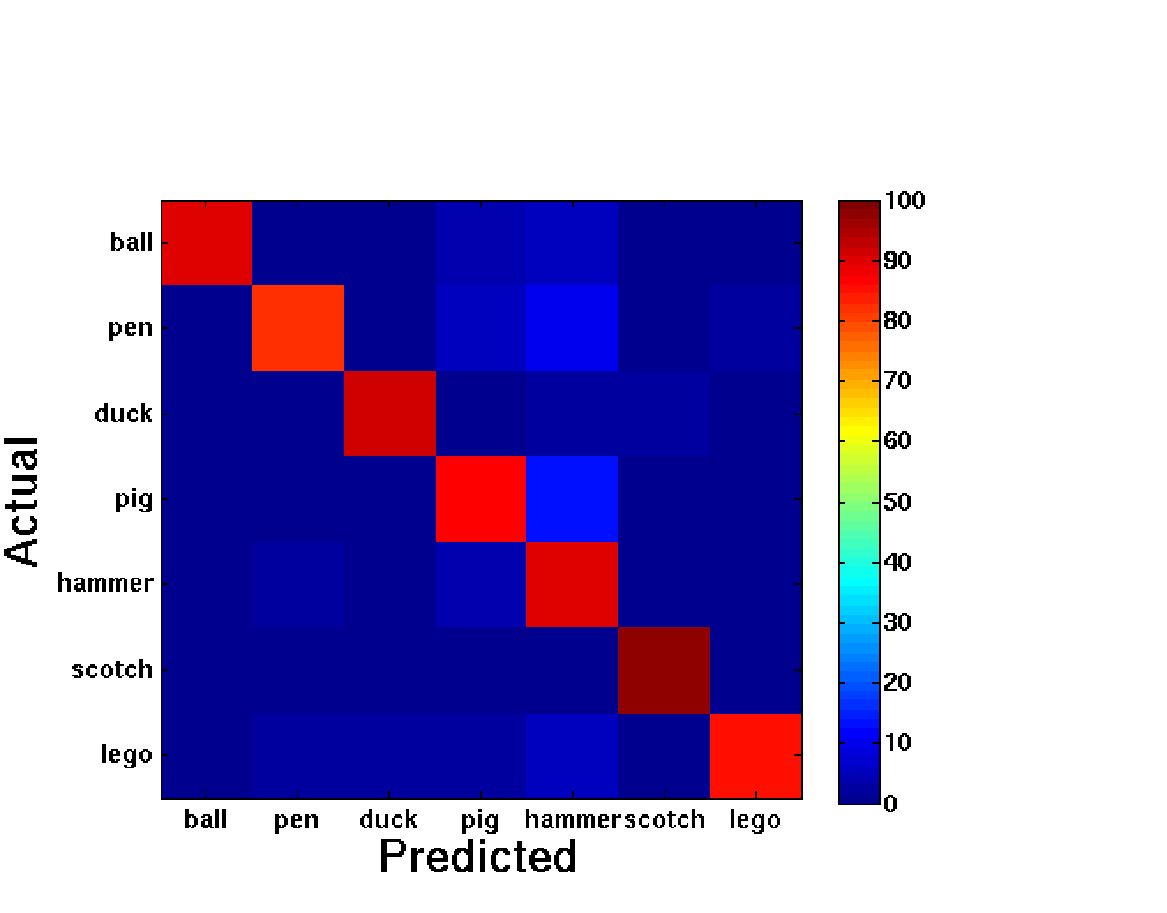
\includegraphics[width=0.25\textwidth]{images/conf_mck_ric.pdf} &
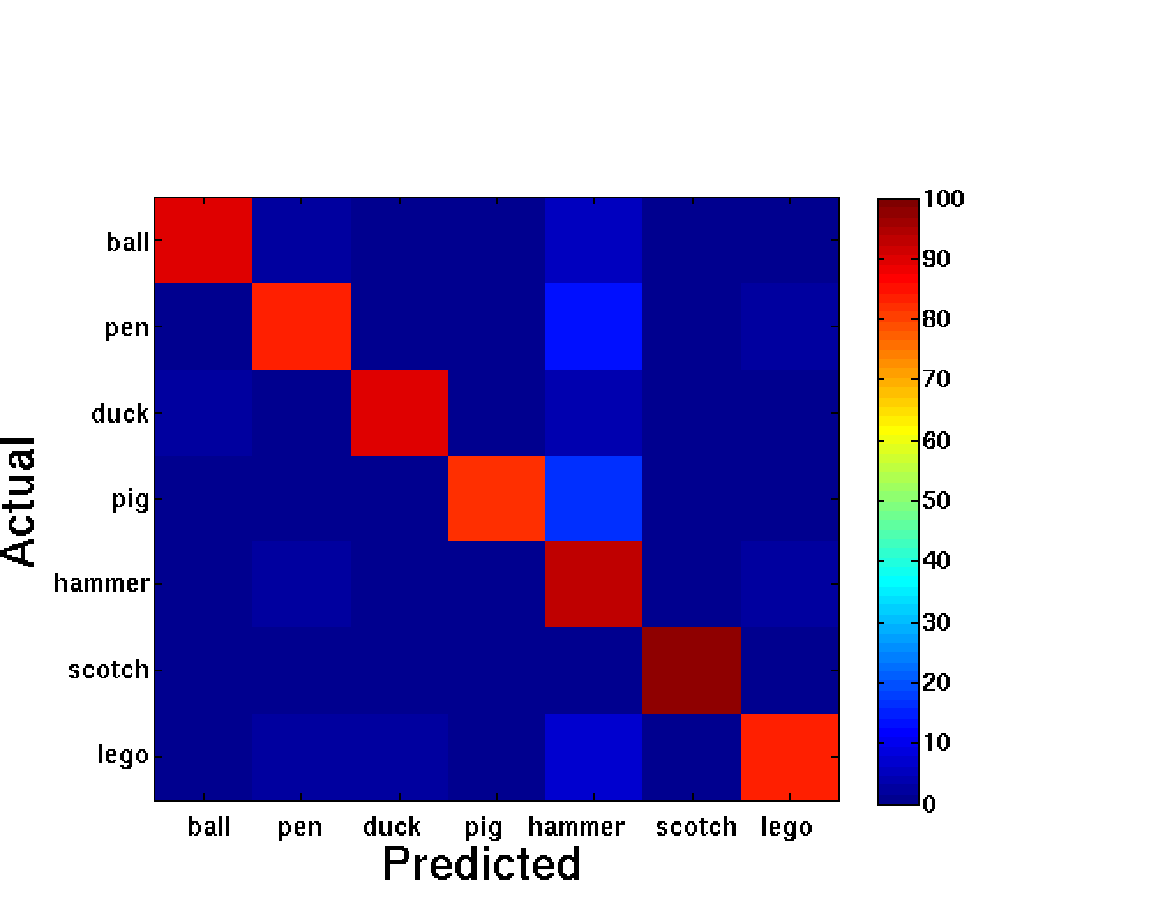
\includegraphics[width=0.25\textwidth]{images/conf_das_ric.pdf} \\
    (d) & (e) & (f)\\
  \end{tabular}
  \caption{(a) Classification mean accuracy of the seven objects averaged
    on the ten splits; (b) confusion matrix using visual features; (c) confusion
    matrix using motor features; (d) confusion matrix using the low-level
    feature integration; (e) confusion matrix using the mid-level
    feature integration; (f) confusion matrix using the high-level
    feature integration.}
  \label{fig:rec_data}
\end{figure*}


Results are reported in Figure \ref{fig:rec_data}. Figure \ref{fig:rec_data}-a shows the recognition rates obtained by using 
only visual information (V -- the same shown in the previous section), only motor information (M), and the two combined together 
(LOW, MID, HIGH). 
We see that using the archetypal grasps as motor information, the performance of the motor only classifier slightly decreases compared to
what we obtained on real motor features: $71.90\%\pm2.06\%$  obtained with the archetypal grasps, as opposed to the
$75.53\%\pm1.22\%$ obtained using real motor features. Still the performance of the multi-modal classifiers show an increase in the overall performance,
compared to the vision only approach.
Once again, the best performance is achieved by MCK (88.77\%$\pm$ 1.29\%), closely followed by DAS (88.38\%$\pm$ 1.31\%).

%Using the motor information we obtain a mean accuracy of $71.90\%\pm2.06\%$, and the mid level integration with the visual features brings to $88.77\%\pm1.29\%$. Overall the combination of the two modalities leads to a statistically significative
%advanatege: the gain in accuracy between MCK and only using visual features is $2.40\%\pm1.05\%$ (difference in accuracy evaluated per split and then averaged on the 10 splits).

Figure \ref{fig:rec_data}-b, -f 
shows the confusion matrices obtained by 
all classifiers, as reported in Section \ref{res:real}.
%the vision only classifier (Figure \ref{fig:rec_data}-b), by the 
%sensorymotor only classifier (Figure \ref{fig:rec_data}-c) and by the MCK classifier (Figure \ref{fig:rec_data}-d). 
We see that the results for the reconstructed motor data are in general lower than that obtained with the
real ones (Figure \ref{fig:real_data}-c). To explain this behaviour there are two things to keep in mind: (1) the lower is the number of
possible grasps associated with an object, the fewer are the data on which the corresponding neural
network is trained; (2) if the first step of hypothesis generation  fails, the error propagates
on the motor data reconstruction. In particular, both points give an intuition about why the objects ``pig'' and ``hammer'' (which were manipulated with only one grasp each) present the worst recognition results using motor
information ($66.65\%$ and $61.45\%$ respectively). Nevertheless, in the ``pig'' case, 
the reconstructed grasp data added to the visual features brings the mean accuracy for object recognition from 
$75.1\%$ (only visual) to $87.0\%$ (using MCK).
As a last remark, we see once again that MCK obtains the best performance (gain in accuracy of $2.40\%$) and therefore it appears to be the most
suitable candidate for the VMC module.





%\subsection{Discussion}
%\label{res:discussion}

%{\bf FIXME BABS: la scrivo quando c'e' un primo draft completo degli esperimenti}

%\begin{itemize}
% \item action dinamic discarded till now
% \item bad visual features, they do not capture the object 3d shape
% \item very simple regression strategy
%\end{itemize}


\section{Conclusions and future work}
\label{sec::conclu}
blabla


%\section{ACKNOWLEDGMENTS}
%
%The authors gratefully acknowledge the contribution of National Research
%Organization and reviewers' comments.

{\small
\bibliographystyle{IEEEtran}
\bibliography{icra10_mirror,icra10_mirror_nic}
}

\end{document}
